Two skaters, Allie and Billie, are at points $A$ and $B$, respectively, on a flat, frozen lake. The distance between $A$ and $B$ is $100$ meters. Allie leaves $A$ and skates at a speed of $8$ meters per second on a straight line that makes a $60^\circ$ angle with $AB$. At the same time Allie leaves $A$, Billie leaves $B$ at a speed of $7$ meters per second and follows the straight path that produces the earliest possible meeting of the two skaters, given their speeds. How many meters does Allie skate before meeting Billie?

\begin{center}
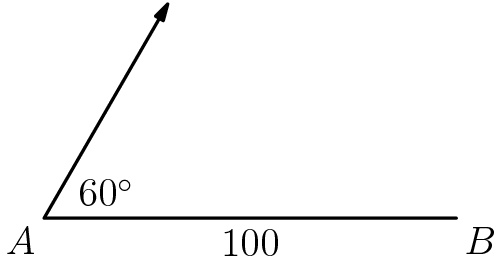
\includegraphics[width = 50.400000000000006mm]{img/fig0.png}
\end{center}